\chapter{Przedstawienie omawianych technologii}
\section{Historia i~rozwój technologii webowych}
Od lat 90 XX wieku świat obserwuje bardzo dynamiczny rozwój technologii związanych z~Internetem. Począwszy od roku 1991, kiedy to naukowcy z~instytu badawczego \textbf{CERN} (ang. \textit{European Organization for Nuclear Research}) opracowali standard WWW, przed programiastami zaczęła się otwierać nowa gałąź tworzenia aplikacji, którą są aplikacje internetowe. Początkowo aplikacje te były jedynie statycznymi stronami WWW, na których znajdował się jedynie tekst. Wprowadzenie kaskadowych arkuszy styli (\emph{CSS}) w~roku 1996 sprawiło, że strony internetowe przybrały graficzną formę. Rok 1997 przyniósł obsługę języka \emph{JavaScript} w~przeglądarkach internetowych. Oznaczało to, że strony internetowe, poza statycznymi elementami, zyskały elementy dynamiczne, np. reagujące na akcje użytkownika.

Wraz ze wzrostem dostępu ludzi do Internetu rozwijały się technologie odpowiedzialne za strony internetowe. Za punkt początkowy istnienia nie stron, a~aplikacji internetowych, można przyjać rok 1997 i~powstanie języka \emph{PHP}. Był to pierwszy interpretowany skryptowy język programowania, który służył do budowania aplikacji internetowych działających w~czasie rzeczywistym. Wraz z~rozwojem języka PHP oraz innych, podobnych mu języków, np. \emph{Python} i~\emph{Ruby}, zmienił się sposób budowania aplikacji. Programiści zaczęli rezygnować ze standardowych klientów w~postaci aplikacji desktopowych i~przechodzili na tzw. cienkich klientów (ang. \textit{thin client}). Trend ten przyspiesza rozwój oraz różnorodność aplikacji serwerowych posiadających interfejs graficzny w~formie strony internetowej, które nazywane są aplikacjami internetowymi \cite{historia}.

\section{Wykorzysywane pojęcia i terminy}
\subsection{Aplikacja internetowa}
Aplikacja internetowa (webowa) jest aplikacją znajdującą się nie na komputerze użytkownika, lecz na ogólnodostępnym serwerze. Komunikacja pomiędzy, niekiedy rozproszonymi, elementami aplikacji odbywa się poprzez sieć komputerową. Aplikacja webowa swój interfejs graficzny poprzez przeglądarkę internetową bądź np. aplikację mobilną.

\subsection{Framework webowy} % moduły i~biblioteki, np do połączenia z~bazą danych
Aby ułatwić korzystanie z~coraz liczniejszych technologii wykorzystywanych w~tworzeniu aplikacji internetowych, powstały narzędzia nazywane frameworkami webowymi. Framework jest uniwersalnym środowiskiem programistycznym, które dostarcza niezbędne narzędzia wymagane do stworzenia aplikacji internetowej w~wybranym języku programowania \cite{framework}. Każdy z~frameworków dostarcza pewną abstrakcję, która znajduje się wokół kodu napisanego przez programistę. Przykładem takiej abstrakcji jest system mapowania ścieżki podstrony (np. \textit{/users/3}) na konkretną akcję w~aplikacji (zwykle akcja \emph{SHOW} dla kontrolera \emph{Users}), czyli \emph{routing}. Twórcy frameworków zauważyli, że w~każdej aplikacji webowej są stosowane te same typy rozwiązań, więc w~wielu przypadkach wprowadzili dane rozwiązania jako integralne części frameworków. W~efekcie programiści mogą korzystać z~gotowych, dogłębnie przetestowanych rozwiązań, które znajdują się w~90\% aplikacji webowych.

\subsection{Wirtualizacja, kontener} % https://dsg.cs.put.poznan.pl/wiki/_media/workshop/docker-skisr.pdf
W celu zapewnienia izolacji środowiska działania aplikacji, stosuję się technikę nazywaną wirtualizacją. Polega ona na stworzeniu wirtualnej maszyny, bądź też kontenera, gdzie uruchamiana jest aplikacja. Rozwiązania te, pomimo osiągania podobnego efektu, różnią się pomiędzy sobą pod wieloma względami.

\begin{figure}[h]
  \centering
  \begin{subfigure}{.5\textwidth}
    \centering
    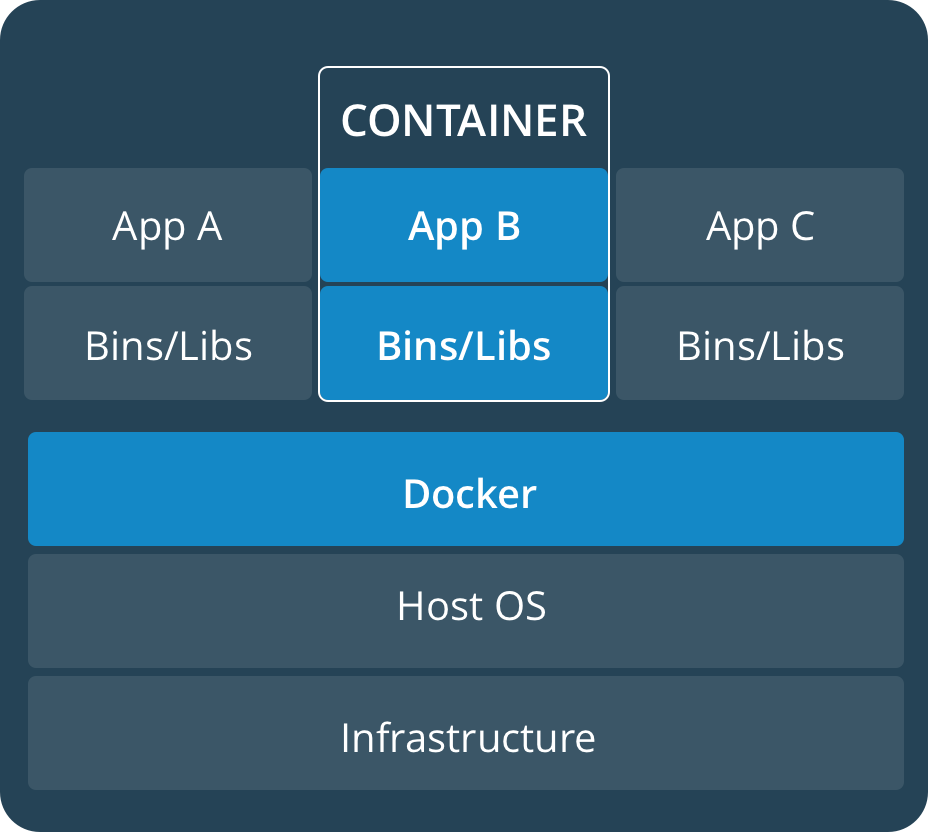
\includegraphics[width=.6\linewidth]{images/docker_container}
    \label{fig:docker_container}
  \end{subfigure}%
  \begin{subfigure}{.5\textwidth}
    \centering
    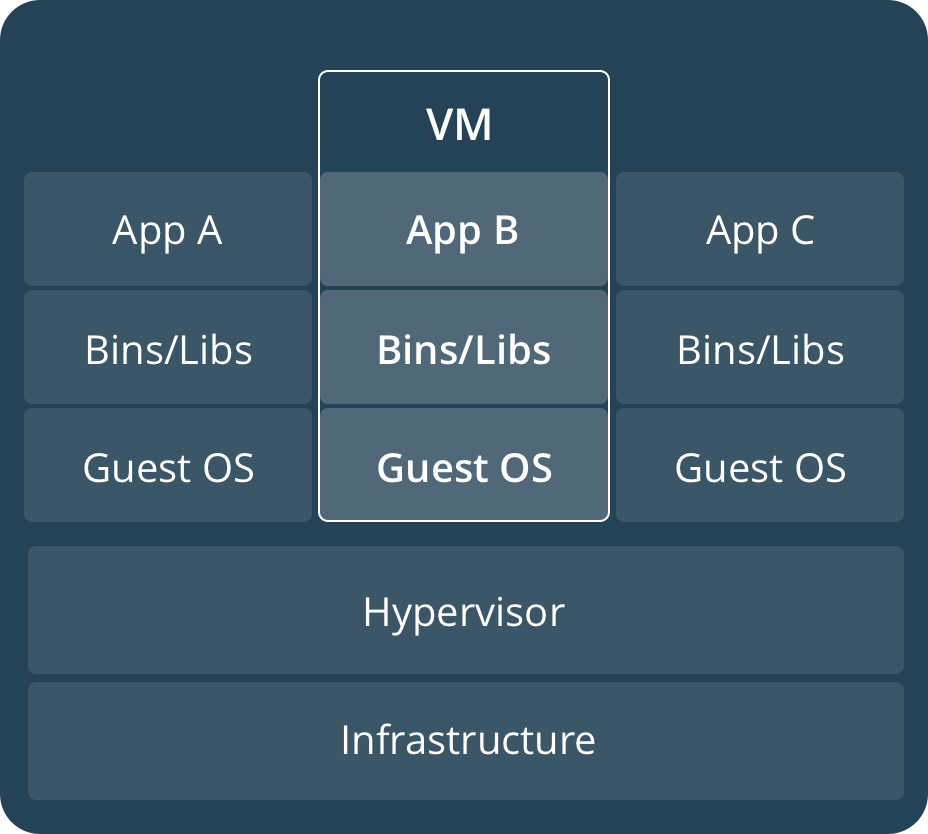
\includegraphics[width=.6\linewidth]{images/docker_vm}
    \label{fig:docker_vm}
  \end{subfigure}
  \caption{Porównanie kontenerów i wirtualnej maszyny.}
\end{figure}

Korzystając z informacji zawartych w dokumentacji Docker'a \cite{docker_what_container}, można wykazać następujące cechy obu rozwiązań:

\begin{itemize}
  \item maszyny wirtualne:
  \begin{itemize}
    \item abstrakcja w warstwie sprzętowej, która zmienia jeden serwer w wiele serwerów,
    \item hipernadzorca (ang. \textit{hypervisor}) pozwala na pracę wielu wirtualnych maszyn na jednej maszynie fizycznej,
    \item każda maszyna wirtualna posiada pełną kopię systemu operacyjnego, aplikacji, niezbędnych bibliotek i ich zależności, przez co zajmuje dużo miejsca na dysku twardym,
    \item maszyny wirtualne zwykle długo się uruchamiają.
  \end{itemize}

  \item kontenery:
  \begin{itemize}
    \item abstrakcja w warstwie aplikacji, która łączy kod z jego zależnościami,
    \item na jednej maszynie może być uruchomionych wiele kontenerów, które wspóldzielą kernel,
    \item każdy z kontenerów jest osobnym procesem w przestrzeni użytkownika,
    \item kontenery zajmują mniej miejsca na dysku i uruchamiają się dużo szybciej, niż maszyny wirtualne.
  \end{itemize}
\end{itemize}

Powyższe zestawienie należy uzupełnić o informacje znajdujące się w prezentacji Łukasza Piątkowskiego \cite{docker_prez}:
\begin{itemize}
  \item maszyny wirtualne:
  \begin{itemize}
    \item wirtualizacja sprzętu - degradacja wydajności,
    \item własny kernel,
    \item pełna maszyna,
  \end{itemize}

  \item kontenery:
  \begin{itemize}
    \item \textit{chroot} z większymi możliwościami,
    \item wspólny kernel,
    \item własne zasoby pamięci, dysku, I/O.
  \end{itemize}
\end{itemize}

Analizując cechy obu rozwiązań można stwierdzić, że kontenery mają sporą przewagę w ważnych kwestiach (wydajność, szybkość uruchamiania, wymagane zasoby) nad maszynami wirtualnymi, dlatego też stają się coraz bardziej popularne.

Ze strony programisty, otrzymuje on nową instancję wybranego systemu, gdzie zainstalowane są jedynie zależności wymagane przez daną aplikację. Prowadzi to do odizolowania środowiska aplikacji, przez co znacząco minimalizowane jest ryzyko wystąpienia konfliktów pomiędzy aplikacjami, aplikację można w bardzo prosty sposób przenieść na inną maszynę i uruchomić ją jedną komendą.

\subsection{CRUD}
CRUD, to cztery podstawowe funkcje w aplikacjach korzystających z pamięci trwałej, które umożliwiają zarządzanie nią \cite{wiki_crud}. Akronim ten powstał od pierwszych liter słów \textbf{C}reate, \textbf{R}ead, \textbf{U}pdate i \textbf{D}elete. Określa on udostępnienie użytkownikowi bądź aplikacji zestaw operacji (stworzenie, odczytanie, aktualizacja oraz usunięcie) na danym obiekcie.
